\section{Universalità I}
Nel 1935 Yukawa predisse l'esistenza di una particella con massa dell'ordine di $100\,\unit{MeV}$ che doveva essere il quanto dell'interazione forte. Una particella di massa simile fu scoperta nel 1938 da Neddermeyer e Anderson nello studio dei raggi cosmici. Nel 1945 Conversi, Pancini e Piccioni giunsero alla conclusione che la particella non poteva essere il quanto della interazione forte. Nel 1947 Muirhead, Lattes e Occhialini scoprirono la catena di decadimento
$$
\pi\to\mu\to e
$$
Nel 1949 Steinberger scoprì che il muone decade in $3$ particelle leggere. Oggi sappiamo che
$$
\mu^-\to e^-+\nu_\mu+\overline{\nu}_e
$$
Da questo momento in poi nasce l'idea che l'interazione di Fermi possa spiegare molti decadimenti in particolare, il decadimento del muone può essere spiegato con il solito diagramma. Cale a dire in modo analogo al decadimento $\beta$ tramite l'interazione delle correnti dell'elettrone e del muone. Occorre pertanto introdurre una corrente per il muone analoga a quella dell'elettrone (quindi bisogna introdurre tanti campi quante sono le particelle che vogliamo descrivere. Per questo nasce l'esigenza di cercare un fattore unificante!)
$$
\hat{J}^\alpha_{(e)} = \overline{\psi}_e \gamma^\alpha (1 - \gamma^5) \psi_{\nu_e} \qquad \hat{J}^\alpha_{(\mu)} = \overline{\psi}_\mu \gamma^\alpha (1 - \gamma^5) \psi_{\nu_\mu}
$$
La corrente leptonica totale diventa
$$
\widehat{L}^\alpha = \widehat{J}^\alpha_{(e)} + \widehat{J}^\alpha_{(\mu)}
$$
Analogamente a quanto già visto la corrente $J^\alpha(\mu)$ crea un muone $\mu^-$ o distrugge un antimuone $\mu^+$ con il campo $\overline{\psi}_\mu$ e distrugge un neutrino $\nu_\mu$ o crea un antineutrino $\overline{\nu}_\mu$ con il campo $\psi_{\nu_\mu}$. Per descrivere la reazione $\mu^-\to e^-+\nu_\mu+\overline{\nu}_e$ dobbiamo distruggere un muone e creare un neutrino. Abbiamo bisogno della corrente $(J^\alpha(\mu))^\dagger$. Possiamo pertanto scrivere l'Hamiltoniana di interazione come
$$
\mathcal{H}' = \frac{G_\mu}{\sqrt{2}} L_\alpha^\dagger L^\alpha
$$
Gli operatori necessari per l'elemento di matrice vengono automaticamente selezionati dagli stati iniziale e finale (a meno di costanti di normalizzazione e spinori)
$$
|i\rangle = |\mu^-\rangle = a_\mu^\dagger |0\rangle \qquad |f\rangle = |e^- \nu_\mu \overline{\nu}_e\rangle = a_e^\dagger a_{\nu_\mu}^\dagger b_{\nu_e}^\dagger |0\rangle
$$
\section{Il decadimento del leptone $\mu$}
Il decadimento del muone è descritto dal solito diagramma. La vita media può essere calcolata con le stesse tecniche utilizzate per il calcolo della vita media del neutrone (si può assumere $m_e=0$). 
$$
\Gamma = \frac{1}{\tau_\mu} = \frac{G_\mu^2 m_\mu^5}{192\pi^3}
$$
La misura della vita media del leptone $\mu$ è molto precisa e permette pertanto una determinazione molto accurata della costante di accoppiamento, per distinguerla da quella ricavata dal decadimento $\beta$ la chiamiamo $G_\mu$. Per poter trarre beneficio dalla precisione della misura sperimentale occorre tenere conto delle correzioni radiative elettromagnetiche che sono descritte dai seguenti diagrammi
\begin{figure}[h!]
	\centering
	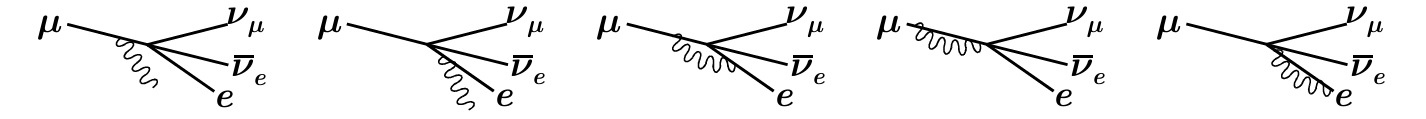
\includegraphics[width=0.6\textwidth]{Lezioni/Lezione 16/corr.png}
	\label{fig:cor}
\end{figure}
Tenendo conto di correzioni $O(\alpha^2)$ e con $m_e\not=0$ si ottiene
$$
\frac{1}{\tau_\mu} = \frac{G_\mu^2 m_\mu^5}{192\pi^3} f \left( \frac{m_e^2}{m_\mu^2} \right) \left[ 1 + \frac{\alpha(m_\mu^2)}{2\pi} \left( \frac{25}{4} - \pi^2 \right) \right]
$$
$$
G_\mu = 1.16637 \pm 0.00001 \times 10^{-5} \, \text{GeV}^{-2} \qquad G_\beta = 1.13578 \pm 0.00027 \times 10^{-5} \, \text{GeV}^{-2}
$$
La quasi identità fra $G_\mu$ e $G_\beta$ è una forte indicazione che la stessa interazione descrive i decadimenti del neutrone $n$ e del muone $\mu$. Ma rimane comunque una differenza significativa rispetto agli errori. Sono comunque molto simili! Interazioni con intensità molto vicina.
\section{Universalità II}
Altri processi che possono essere spiegati con estensioni dell'Hamiltoniana del decadimento $\beta$ che abbiamo studiato:
\begin{itemize}
	\item Decadimenti e urti completamente leptonici
	$$
	\mu^- \to e^- + \nu_\mu + \overline{\nu}_e \quad \quad \tau^- \to e^- + \nu_\tau + \overline{\nu}_e \quad \quad \nu_e + e^- \to \nu_e + e^-
	$$
	$$
	\tau^- \to \mu^- + \nu_\tau + \overline{\nu}_\mu
	$$
	\item Decadimenti e urti semi-leptonici senza variazione di Stranezza
	$$
	n \to p + e^- + \overline{\nu}_e \quad \quad \pi^- \to \pi^0 + e^- + \overline{\nu}_e \quad \quad \pi^- \to \mu^- + \overline{\nu}_\mu
	$$
	$$
	\Sigma^\pm \to \Lambda + l^\pm + \nu_l \quad \quad \nu_\mu + N \to \mu^- + X \quad \quad \tau^- \to \pi^- + \nu_\tau
	$$
	\item Decadimenti semi-leptonici con variazione di Stranezza
	$$
	K^- \to \mu^- + \overline{\nu}_\mu \quad \quad K^- \to \pi^0 + e^- + \overline{\nu}_e \quad \quad \Lambda^0 \to p + e^- + \overline{\nu}_e
	$$
	\item Decadimenti totalmente adronici con variazione di Stranezza
	$$
	\Lambda \to p + \pi^- \quad \quad \Sigma^+ \to p + \pi^0 \quad \quad K^0 \to \pi^+ + \pi^-
	$$
\end{itemize}
Tutti questi decadimenti sono stati studiati con successo e hanno confermato la validità della interazione fra due correnti.
\section{La corrente adronica}
Nello studio del decadimento beta abbiamo utilizzato l'operatore corrente adronica 
$$
\hat{J}^\mu (h) = \overline{\hat{\psi}}_n \gamma^\mu (1 - \kappa \gamma^5) \hat{\psi}_p
$$
Ne abbiamo calcolato l'elemento di matrice fra due stati (il neutrone iniziale e il protone finale). Abbiamo inoltre notato che il fattore $\kappa$ diverso da $1$ è dovuto al fatto che gli adroni non sono puntiformi. Pertanto occorre tenere conto dell'interazione forte. Nello studio delle correnti degli adroni risulta conveniente utilizzare una corrente $\hat{\mathfrak{J}}^\mu$ generica (non definita esplicitamente). Questo è un operatore vettoriale (nel senso di Lorentz). Dagli esperimenti abbiamo visto che deve avere una parte vettoriale e una assiale
$$
\hat{\mathfrak{J}}^\mu = \hat{V}^\mu + \hat{A}^\mu
$$
Gli esperimenti ci dicono quali regole di selezione deve riprodurre. Per il calcolo delle quantità osservabili occorre calcolare l'elemento di matrice dell'operatore fra stati di particelle. Ad esempio, nel caso del decadimento $\beta$ del neutrone si ha
$$
\langle p, k_p, s_p \mid \hat{\mathfrak{J}}^\mu \mid n, k_n, s_n \rangle = F^\mu (k_p, s_p, k_n, s_n)
$$
Le funzioni $F^\mu$ sono un insieme di c-numbers (non sono operatori). A seconda del tipo di accoppiamento ipotizzato le funzioni $F^\mu$ hanno uno (o più, o zero) indici di Lorentz. In dipendenza dalla natura degli stati (iniziale e finale) le funzioni $F^\mu$ hanno come argomenti $4-$momenti e variabili di spin. Complessivamente hanno ben precise proprietà di trasformazione per trasformazioni di Lorentz. Utilizzando le proprietà di invarianza (di Lorentz) e le regole di selezione si può scrivere la forma più generale dell'elemento di matrice e confrontarlo con i dati sperimentali per determinare le parti incognite (ad esempio l'origine del fattore $\kappa\approx1.26$). Spieghiamo meglio con un esempio: il decadimento $\pi^-\to l^-\overline{\nu}_l$
\section{Il decadimento $\pi^-\to l^- \overline{\nu}_l$}
Il mesone $\pi$ predetto da Yukawa e scoperto da Neddarmeyer e Anderson è l'adrone più leggero. Non può decadere tramite interazione forte e decade tramite interazione debole
$$
\pi^- \to \mu^- + \overline{\nu}_\mu \quad \quad \pi^- \to e^- + \overline{\nu}_e \quad \quad \pi^- \to \pi^0 + e^- + \overline{\nu}_e
$$
Il decadimento è rappresentato schematicamente dal diagramma
\begin{figure}[h!]
	\centering
	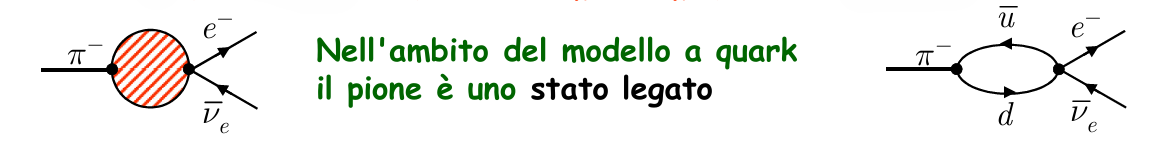
\includegraphics[width=0.8\textwidth]{Lezioni/Lezione 16/ty.png}
	\label{fig:ty}
\end{figure}
Nel diagramma con i quark non è nota la struttura dello stato legato e i quark interagiscono tramite gluoni (QCD): non trattabile perturbativamente. Si ipotizza una interazione corrente-corrente fra la corrente leptonica e la generica corrente adronica $\mathfrak{J}^\mu$
$$
\mathcal{H}' = \frac{G}{\sqrt{2}} (\mathfrak{J}^\mu)^\dagger L_\mu
$$
Lo stato iniziale e lo stato finale sono
$$
|i\rangle = |\pi^-\rangle \quad \quad |f\rangle = |l^- \overline{\nu}_l\rangle
$$
L'elemento di matrice è
$$
\langle f | \mathcal{H}' | i \rangle = \langle l^- \overline{\nu}_l | \mathcal{H}' | \pi^- \rangle
$$
Per gli adroni si passa da uno stato con un pione allo stato vuoto (nel caso del decadimento $\beta$ si passa dal neutrone al protone). Per i leptoni, come nel caso del decadimento $\beta$ si passa da uno stato vuoto allo stato con due leptoni. Si può procedere come nel caso del decadimento $\beta$ per giungere alla seguente espressione per l'ampiezza.
$$
\mathfrak{M} = \frac{G_\beta}{\sqrt{2}} \langle 0 | \mathfrak{J}^\mu (0) | \pi^- \rangle \langle l^- \overline{\nu}_l | L_\mu (0) | 0 \rangle
$$
La parte leptonica è identica a quanto visto per il decadimento $\beta$
$$
\langle l^- \overline{\nu}_l | L^\mu (0) | 0 \rangle = \overline{u}_l (k_l) \gamma_\mu (1 - \gamma^5) v_\nu (k_\nu)
$$
Consideriamo la parte adronica. Deve essere proporzionale a $p^\mu$, il $4-$momento del pione che è l'unico che può portare l'indice di Lorentz
$$
\langle 0 | \mathfrak{J}^\mu (0) | \pi^- \rangle = f p^\mu
$$
La costante di proporzionalità $f$ deve essere una funzione invariante e quindi può solo dipendere da quantità invarianti $p^2=m^2$. Pertanto $f(p^2)=f_\pi$ è una costante ma non abbiamo nessun modo per prevederlo per questo è un modello fenomenologico e lo misuriamo in un esperimento come se fosse una costante di accoppiamento!
$$
\langle 0 | \mathfrak{J}^\mu (0) | \pi^- \rangle = f_\pi p^\mu
$$
Per la conservazione del $4-$momento totale abbiamo $p^\mu=k_l^\mu+k_\nu^\mu$. La quantità $f_\pi$ è una costante che dipende dalla natura del mesone che decade e ha le dimensioni di una energia. L'elemento di matrice diventa pertanto
$$
\mathfrak{M} = \frac{G_\beta}{\sqrt{2}} f_\pi \overline{u}_l (k_l) p^\mu \gamma_\mu (1 - \gamma^5) v_\nu (k_\nu) \qquad p^\mu \gamma_\mu = \slashed{p} = \slashed{k}_l + \slashed{k}_\nu
$$
Si può ulteriormente semplificare ricordando che
$$
(\slashed{k} - m)u = 0 \quad \quad (\slashed{k} + m)v = 0
$$
$$
\overline{u}(\slashed{k} - m) = 0 \quad \quad \overline{v}(\slashed{k} + m) = 0
$$
Pertanto
$$
\mathfrak{M} = \frac{G_\beta}{\sqrt{2}} f_\pi \overline{u}_l (k_l) (\slashed{k}_l + \slashed{k}_\nu) (1 - \gamma^5) v_\nu (k_\nu) = \frac{G_\beta}{\sqrt{2}} f_\pi m_l \overline{u}_l (k_l) (1 - \gamma^5) v_\nu (k_\nu)
$$
Si può notare che esce la massa del leptone che prima non c'era ($m_l$) ma da dove arriva? Perché c'era il $\slashed{k}$ ma da dove deriva? Deriva dal fatto che c'è l'accoppiamento vettoriale $\gamma^\mu$. Il modulo quadrato sommato sulle polarizzazioni dello stato finale si ottiene con le usuali tracce
$$
\overline{|\mathfrak{M}|^2} = \frac{G_\beta^2}{2} f_\pi^2 m_l^2 \text{Tr} \left[ (\slashed{k}_l + m_l)(1 - \gamma^5) \slashed{k}_\nu (1 + \gamma^5) \right]
$$
La traccia si calcola facilmente
$$
\begin{aligned}
	\text{Tr} \left[ (\slashed{k}_l + m_l)(1 - \gamma^5) \slashed{k}_\nu (1 + \gamma^5) \right] &= \text{Tr} \left[ (\slashed{k}_l + m_l)(1 - \gamma^5)^2 \slashed{k}_\nu \right] \\
	&= 2 \text{Tr} \left[ (\slashed{k}_l + m_l)(1 - \gamma^5) \slashed{k}_\nu \right] \\
	&= 2 \text{Tr} [\slashed{k}_l \slashed{k}_\nu] = 8 k_l \cdot k_\nu
\end{aligned}
$$
Si ha inoltre
$$
m_\pi^2 = p^2 = (k_l + k_\nu)^2 = k_l^2 + 2 k_l \cdot k_\nu + k_\nu^2 \qquad k_\nu^2 = m_\nu^2 = 0 \qquad k_l \cdot k_\nu = \frac{m_\pi^2 - m_l^2}{2}
$$
In conclusione
$$
\overline{|\mathfrak{M}|^2} = 2 G_\beta^2 f_\pi^2 m_l^2 (m_\pi^2 - m_l^2)
$$
Notiamo che l'elemento di matrice è costante, come ci si poteva attendere. La larghezza di decadimento è
$$
\Gamma = \int \frac{\overline{|\mathfrak{M}|^2}}{2m_\pi} d\Phi_2 = \frac{\overline{|\mathfrak{M}|^2}}{2m_\pi} \int d\Phi_2
$$
ricordiamo lo spazio delle fasi per uno stato finale di due particelle nel C.M. del $\pi$
$$
d\Phi_2 = \frac{1}{(4\pi)^2} \delta(W_i - W_f) \frac{|\mathbf{p}_f|}{W_f} dW_f d\Omega \quad \quad |\mathbf{p}_f| = \frac{m_\pi^2 - m_l^2}{2m_\pi} \quad \quad W_f = m_\pi
$$
L'integrale è banale
$$
\int d\Phi_2 = \frac{1}{(4\pi)^2} \int \delta(W_i - W_f) \frac{|\mathbf{p}_f|}{W_f} dW_f d\Omega = \frac{1}{(4\pi)^2} \int \frac{m_\pi^2 - m_l^2}{2m_\pi} \frac{1}{m_\pi} d\Omega
$$
$$
\int d\Phi_2 = \frac{1}{4\pi} \frac{m_\pi^2 - m_l^2}{2m_\pi^2}
$$
In linea di principio tanto più grande è lo spazio delle fasi tanto è più probabile un decadimento ma noi vedremo che per questo caso specifico è esattamente il contrario. In definitiva otteniamo per la larghezza di decadimento 
$$
\Gamma = \frac{1}{\tau} = \frac{\overline{|\mathfrak{M}|^2}}{2m_\pi} \int d\Phi_2 \qquad \Gamma = \frac{1}{2m_\pi} 2 G_\beta^2 f_\pi^2 m_l^2 (m_\pi^2 - m_l^2) \frac{1}{4\pi} \frac{m_\pi^2 - m_l^2}{2m_\pi^2}
$$
$$
\Gamma = \frac{G_\beta^2}{8\pi} f_\pi^2 m_l^2 m_\pi \left( 1 - \frac{m_l^2}{m_\pi^2} \right)^2
$$
Il pione decade circa nel $100\%$ dei casi in muone ed ha una vita media
$$
\tau = 2.6033 \pm 0.0005 \times 10^{-8} \, \text{s}
$$
Da questo valore si può ricavare il parametro fenomenologico $f_\pi$
$$
f_\pi = 130.7 \pm 0.1 \, \text{MeV}
$$
Questo $f_\pi$ lo possiamo trovare in tantissimi altri calcoli in cui non centra direttamente questa costante allora questo acquista potere predittivo per altri processi.

Il decadimento in elettrone è molto raro e la misura della frazione di decadimento dà
$$
\frac{\Gamma(\pi \to e\nu)}{\Gamma(\pi \to \mu\nu)} = 1.230 \pm 0.004 \times 10^{-4}
$$
Questo rapporto prende il nome di inflazione di decadimento. Questo ci dice che ogni diecimila decadimenti del $\pi$ c'è solo un decadimento in elettrone mentre gli altri in muone.
Va confrontata con il risultato del nostro calcolo
$$
R = \frac{\Gamma(\pi \to e\nu)}{\Gamma(\pi \to \mu\nu)} = \frac{m_e^2 (m_\pi^2 - m_e^2)^2}{m_\mu^2 (m_\pi^2 - m_\mu^2)^2} \quad \quad R = 1.283 \times 10^{-4}
$$
Vediamo che il nostro calcolo riproduce "bene" il valore sperimentale (perché è un calcolo solo al primo ordine). L'ingrediente chiave è la massa del leptone la cui origine è dovuta all'accoppiamento di tipo vettoriale ($\gamma^\mu$ oppure $\gamma^5\gamma^\mu$).
\section{Polarizzazione del leptone}
Come nel caso del decadimento $\beta$ del neutrone è facile calcolare la polarizzazione del leptone carico nel decadimento del pione (calcoli in cui si va veloce)
$$
\overline{|\mathfrak{M}_{RL}|^2} = \frac{G_\beta^2}{2} f_\pi^2 m_l^2 \text{Tr} \left[ (\slashed{k}_l + m_l) \frac{1 \pm \gamma^5 \slashed{s}_R}{2} (1 - \gamma^5) \slashed{k}_\nu (1 + \gamma^5) \right]
$$
Otteniamo pertanto
$$
\overline{|\mathfrak{M}_R|^2} - \overline{|\mathfrak{M}_L|^2} = \frac{G_\beta^2}{2} f_\pi^2 m_l^2 \text{Tr} \left[ (\slashed{k}_l + m_l) \gamma^5 \slashed{s}_R (1 - \gamma^5) \slashed{k}_\nu (1 + \gamma^5) \right]
$$
Si verifica facilmente che
$$
\text{Tr} \left[ (\slashed{k}_l + m_l) \gamma^5 \slashed{s}_R (1 - \gamma^5) \slashed{k}_\nu (1 + \gamma^5) \right] = 8m_l s_R \cdot k_\nu
$$
Il vettore di polarizzazione longitudinale del leptone è
$$
s_R = \left( \frac{|\mathbf{k}_l|}{m_l}, \frac{E_l}{m_l} \frac{\mathbf{k}_l}{|\mathbf{k}_l|} \right)
$$
Dalla cinematica si ottiene facilmente
$$
|\mathbf{k}_l| = \frac{m_\pi^2 - m_l^2}{2m_\pi} \quad \quad E_l = \frac{m_\pi^2 + m_l^2}{2m_\pi} \qquad k_\nu = (|\mathbf{k}_l|, -\mathbf{k}_l) \quad \quad k_\nu \cdot s_R = \frac{|\mathbf{k}_l|^2}{m_l} \left( 1 + \frac{E_l}{|\mathbf{k}_l|} \right)
$$
Ribadiamo
$$
\overline{|\mathfrak{M}_R|^2} + \overline{|\mathfrak{M}_L|^2} = \overline{|\mathfrak{M}|^2} = 2G_\beta^2 f_\pi^2 m_l^2 (m_\pi^2 - m_l^2)
$$
In definitiva
$$
\frac{\overline{|\mathfrak{M}_R|^2} - \overline{|\mathfrak{M}_L|^2}}{\overline{|\mathfrak{M}_R|^2} + \overline{|\mathfrak{M}_L|^2}} = \frac{2\mathbf{k}_l^2}{m_\pi^2 - m_l^2} \left( 1 + \frac{E_l}{|\mathbf{k}_l|} \right) = 2 \frac{(m_\pi^2 - m_l^2)^2}{4m_\pi^2 (m_\pi^2 - m_l^2)} \frac{2m_\pi^2}{m_\pi^2 - m_l^2} = 1
$$
Il risultato precedente mostra che nel sistema di riposo del pione il leptone è polarizzato al $100\%$ nella sua direzione di moto. La polarizzazione non $-\beta$ come avevamo visto per i decadimenti con interazione debole. Questo risultato era prevedibile per i seguenti motivi:
\begin{itemize}
	\item Il pione ha spin $0$
	\item L'antineutrino è right-handed (particella con massa nulla quindi polarizzata al $100\%$)
	\item Per la conservazione del momento angolare anche il leptone carico è right-handed per far in modo che il momento angolare totale sia zero in quanto il pione è una particella scalare.
\end{itemize}
Questo spiega qualitativamente perchè il decadimento in elettrone è molto più raro nonostante dovrebbe essere favorito per lo spazio delle fasi
$$
\int d\Phi_2 = \frac{1}{4\pi} \frac{m_\pi^2 - m_l^2}{2m_\pi^2} \qquad \int d\Phi_2 = 0.04 \quad (e^-) \quad \quad \int d\Phi_2 = 0.017 \quad (\mu^-)
$$
La conservazione del momento angolare obbliga il leptone a essere emesso con la polarizzazione "sbagliata" (rispetto a quella imposta dalla corrente $V-A$). Per l'elettrone (che è molto più leggero e che ha un $\beta\approx1$) ciò è molto difficile (probabilità $1-\beta$) infatti l'elettrone che esce da un decadimento $\beta$ ha un'energia dell'ordine di $\sim100\,\unit{MeV}$. Se il leptone avesse massa nulla il decadimento avrebbe larghezza nulla.
\section{Il decadimento del leptone $\tau$}
Mostriamo come il formalismo fin qui sviluppato può essere utilizzato anche per il calcolo della frazione di decadimento del leptone $\tau$ nel mesone $\pi$. Visto che il $\tau$ è una particella molto massiva $m_\tau\approx 1777\,\unit{MeV}$ ha moltissimi canali possibili di decadimento. Osserviamo prima di tutto che per il calcolo della vita media o della larghezza di decadimento occorrerebbe calcolare tutte le larghezze parziali
$$
\tau^- \to l^- + \overline{\nu}_l + \nu_\tau \quad \quad \tau^- \to h^- + \nu_\tau \quad \quad h = \pi, K, \rho, a_1 \quad \quad \tau^- \to (n\pi)^- + \nu_\tau
$$
$$
\Gamma = \Gamma_{e\nu\nu} + \Gamma_{\mu\nu\nu} + \Gamma_{\pi\nu} + \dots + \Gamma_{K\nu}
$$
Troppo lavoro... Calcoliamo solo la larghezza del decadimento in $\pi^-$ $\nu_\tau$ e confrontiamola con la larghezza totale. La larghezza totale può essere derivata dalla vita media. Dal risultato sperimentale $\tau=290.6\times10^{-15}\,\unit{s}$ ricaviamo
$$
\Gamma(\tau \to all) = \frac{\hbar}{\tau} = \frac{6.582 \times 10^{-22} \, \text{MeV s}}{290.6 \times 10^{-15} \, \text{s}} \qquad \Gamma(\tau \to all) = 2.265 \times 10^{-3} \, \text{eV}
$$
Calcoliamo adesso la larghezza del decadimento $\pi^-\nu_\tau$. Il calcolo è identico a quello fatto per il decadimento del pione. Si utilizza l'Hamiltoniana
$$
\mathcal{H}' = \frac{G}{\sqrt{2}} (\mathfrak{J}^\mu)^\dagger J_\mu
$$
La corrente leptonica $J^\mu$ adesso contiene anche un termine per il leptone $\tau$. Lo stato iniziale e lo stato finale sono rispettivamente 
$$
|\tau^-\rangle \quad \quad |\pi^- \nu_\tau\rangle
$$
Notiamo in particolare che per quel che riguarda gli adroni si passa dallo stato vuoto allo stato con un pione. La situazione opposta a quella del decadimento del pione. Scriviamo pertanto l'ampiezza di decadimento
$$
\mathfrak{M} = \frac{G_\beta}{\sqrt{2}} \langle \pi^- \mid \mathfrak{J}^\mu (0) \mid 0 \rangle \langle \nu_\tau \mid J_\mu (0) \mid \tau^- \rangle
$$
L'elemento di matrice della parte adronica è il complesso coniugato di quello che avevamo nel decadimento del pione. Dato che era reale sono uguali
$$
\langle \pi^- \mid \mathfrak{J}^\mu (0) \mid 0 \rangle = f_\pi q^\mu
$$
Qui vediamo il significato del discorso fatto prima: abbiamo fatto un calcolo che ci ha permesso di ricavare $f_\pi$ e ora possiamo usarlo per altri calcoli in cui in qualche modo si introduce lo stesso elemento di matrice. Ma la cinematica è diversa infatti: il $4-$vettore $q^\mu$ è il momento del pione $q^\mu=k_\tau^\mu-k_\nu^\mu$. L'elemento di matrice della parte leptonica è
$$
\langle \nu_\tau \mid J^\mu (0) \mid \tau^- \rangle = \overline{u}_\nu (k_\nu) \gamma_\mu (1 - \gamma^5) u_\tau (k_\tau)
$$
Per finire l'ampiezza è
$$
\mathfrak{M} = \frac{G_\beta}{\sqrt{2}} f_\pi \overline{u}_\nu (k_\nu) q^\mu \gamma_\mu (1 - \gamma^5) u_\tau (k_\tau)
$$
Sostituendo $q^\mu=k_\tau^\mu-k_\nu^\mu$
$$
\mathfrak{M} = \frac{G_\beta}{\sqrt{2}} f_\pi \overline{u}_\nu (k_\nu) (\slashed{k}_\tau - \slashed{k}_\nu) (1 - \gamma^5) u_\tau (k_\tau) = \frac{G_\beta}{\sqrt{2}} f_\pi m_\tau \overline{u}_\nu (k_\nu) (1 + \gamma^5) u_\tau (k_\tau)
$$
Con la solita tecnica troviamo
$$
\overline{|\mathfrak{M}|^2} = \frac{G_\beta^2}{2} f_\pi^2 m_\tau^2 \text{Tr} \left[ (\slashed{k}_\nu)(1 + \gamma^5)(\slashed{k}_\tau + m_\tau)(1 - \gamma^5) \right]
$$
$$
= G_\beta^2 f_\pi^2 m_\tau^2 \text{Tr} \left[ (\slashed{k}_\nu)(\slashed{k}_\tau + m_\tau)(1 - \gamma^5) \right] = G_\beta^2 f_\pi^2 m_\tau^2 \text{Tr} [\slashed{k}_\nu \slashed{k}_\tau] = 4 G_\beta^2 f_\pi^2 m_\tau^2 k_\nu \cdot k_\tau
$$
Dalla cinematica otteniamo
$$
k_\tau \cdot k_\nu = \frac{m_\tau^2 - m_\pi^2}{2} \quad \quad \int d\Phi_2 = \frac{1}{4\pi} \frac{m_\tau^2 - m_\pi^2}{2m_\tau^2}
$$
Mettendo insieme i vari pezzi otteniamo
$$
\Gamma = \frac{1}{\tau} = \frac{\frac{1}{2}\overline{|\mathfrak{M}|^2}}{2m_\tau} \int d\Phi_2 \qquad \Gamma = \frac{1}{4m_\tau} 4G_\beta^2 f_\pi^2 m_\tau^2 \frac{m_\tau^2 - m_\pi^2}{2} \frac{1}{4\pi} \frac{m_\tau^2 - m_\pi^2}{2m_\tau^2}
$$
$$
\Gamma(\tau \to \pi\nu) = \frac{1}{16\pi} G_\beta^2 f_\pi^2 m_\tau^3 \left( 1 - \frac{m_\pi^2}{m_\tau^2} \right)^2
$$
Notiamo il fattore $\frac{1}{2}$ introdotto prima dell'elemento di matrice. Questa volta il leptone è nello stato iniziale e quindi bisogna mediare statisticamente fra le due polarizzazioni possibili. Introduciamo i valori delle costanti e delle masse
$$
G_\beta = 1.13578 \pm 0.00027 \times 10^{-5} \, \text{GeV}^{-2} \quad \quad m_\pi = 139.57018 \pm 0.00035 \, \text{MeV}
$$
$$
f_\pi = 130.7 \pm 0.1 \, \text{MeV} \quad \quad m_\tau = 1776.99 \pm 0.29 \, \text{MeV}
$$
Otteniamo
$$
\Gamma(\tau \to \pi\nu) = 2.43 \times 10^{-4} \, \text{eV}
$$
Ricordando la larghezza totale ottenuta dalla vita media
$$
\Gamma (\tau \to all) = 2.265 \times 10^{-3} \text{ eV}
$$
Otteniamo la frazione di decadimento
$$
\frac{\Gamma (\tau \to \pi\nu)}{\Gamma (\tau \to all)} = \frac{2.43 \times 10^{-4}}{2.265 \times 10^{-3}} = 10.7\%
$$
Da confrontare con il valore sperimentale
$$
\frac{\Gamma (\tau \to \pi\nu)}{\Gamma (\tau \to all)} = 11.06 \pm 0.11\%
$$
Ancora una volta, un ottimo accordo per un calcolo al primo ordine.
\section{Polarizzazione del leptone $\tau$}
Calcoliamo adesso la larghezza di decadimento nel caso in cui il leptone $\tau$ sia polarizzato. Questo ci permette di vedere come la materia e l'antimateria si comporta in maniera diversa. L'ampiezza mediata
$$
\overline{|\mathfrak{M}|^2} = \frac{G_\beta^2}{2} f_\pi^2 m_\tau^2 \text{Tr} [(\slashed{k}_\nu)(1 + \gamma^5)(\slashed{k}_\tau + m_\tau)(1 - \gamma^5)]
$$
Viene sostituita con l'espressione
$$
\overline{|\mathfrak{M}_{RL}|^2} = \frac{G_\beta^2}{2} f_\pi^2 m_\tau^2 \text{Tr} \left[ \slashed{k}_\nu (1 + \gamma^5) (\slashed{k}_\tau + m_\tau) \frac{1 \pm \gamma^5 \slashed{s}_R}{2} (1 - \gamma^5) \right]
$$
$$
\overline{|\mathfrak{M}_R|^2} = \frac{1}{2} G_\beta^2 f_\pi^2 m_\tau^2 \text{Tr} [ \slashed{k}_\nu (\slashed{k}_\tau + m_\tau) (1 + \gamma^5 \slashed{s}_R) (1 - \gamma^5) ] = \frac{1}{2} G_\beta^2 f_\pi^2 m_\tau^2 \text{Tr} [\slashed{k}_\nu \slashed{k}_\tau + m_\tau \slashed{k}_\nu \slashed{s}_R]
$$
Visto che ho una particella ho $+m_\tau$.
$$
= 2 G_\beta^2 f_\pi^2 m_\tau^2 (k_\tau \cdot k_\nu + m_\tau s_R \cdot k_\nu)
$$
Adesso mettiamoci nel sistema di riposo del leptone
$$
s_R = (0, \boldsymbol{\xi}) \quad \quad \mathbf{k}_\pi = -\mathbf{k}_\nu \quad \quad |\mathbf{k}_\nu| = \frac{m_\tau^2 - m_\pi^2}{2m_\tau}
$$
$$
\overline{|\mathfrak{M}_R|^2} = 2 G_\beta^2 f_\pi^2 m_\tau^2 (m_\tau E_\nu - m_\tau \boldsymbol{\xi} \cdot \mathbf{k}_\nu) = 2 G_\beta^2 f_\pi^2 m_\tau^2 (m_\tau E_\nu - m_\tau E_\nu \boldsymbol{\xi} \cdot \hat{\mathbf{k}}_\nu)
$$
$$
= 2 G_\beta^2 f_\pi^2 m_\tau^3 E_\nu (1 + \boldsymbol{\xi} \cdot \hat{\mathbf{k}}_\pi)
$$
$$
\overline{|\mathfrak{M}_{RL}|^2} = 2 G_\beta^2 f_\pi^2 m_\tau^3 E_\nu (1 \pm \boldsymbol{\xi} \cdot \hat{\mathbf{k}}_\pi)
$$
Si ottiene infine la distribuzione angolare dei pioni nel sistema di riposo del leptone $\tau$
$$
\frac{dN_{RL}}{d\Omega} = \frac{\Gamma_{RL}}{\Gamma_R + \Gamma_L}
$$
Nel rapporto i termini costanti dello spazio delle fasi si elidono e pertanto possiamo semplicemente fare il rapporto fra i quadrati delle ampiezze
$$
\frac{dN_{RL}}{d \cos \theta^*} = \frac{\overline{|\mathfrak{M}_{RL}|^2}}{\overline{|\mathfrak{M}_R|^2} + \overline{|\mathfrak{M}_L|^2}} \qquad \frac{dN_{RL}}{d \cos \theta^*} = \frac{1}{2} (1 \pm \boldsymbol{\xi} \cdot \hat{\mathbf{k}}_\pi)
$$
$$
\frac{dN_{RL}}{d \cos \theta^*} = \frac{1}{2} (1 \pm |\boldsymbol{\xi}| \cos \theta^*)
$$
Osserviamo infine che il segno di fronte al prodotto $\xi\cdot k_\nu$ dipende dal segno della massa nell'espressione
$$
\overline{|\mathfrak{M}_R|^2} = \frac{1}{2} G_\beta^2 f_\pi^2 m_\tau^2 \text{Tr} [\slashed{k}_\nu (\slashed{k}_\tau + m_\tau)(1 + \gamma^5 \slashed{s}_R)(1 - \gamma^5)] = 2 G_\beta^2 f_\pi^2 m_\tau^2 (k_\tau \cdot k_\nu + m_\tau s_R \cdot k_\nu)
$$
La massa compare con questo segno perchè nell'ampiezza era presente lo spinore $u$ del $\tau^-$ (particella). Se invece ci fosse stato un $\tau^+$ (antiparticella) allora ci sarebbe stato uno spinore $v$ e quindi una massa con il segno opposto.
\section{Decadimento deboli}
Abbiamo visto che l'interazione di Fermi (interazione corrente-corrente) può essere utilizzata con successo per descrivere i decadimenti deboli. Assumendo l'universalità l'Hamiltoniana può essere scritta come
$$
\mathcal{H}'(x) = \frac{G}{\sqrt{2}} \mathcal{J}^{\dagger \alpha} (x) \mathcal{J}_\alpha (x) \quad \quad G \equiv G_\mu
$$
La corrente $\mathcal{J}^\alpha(x)$ è fatta da due pezzi:
$$
\mathcal{J}^\alpha(x) = l^\alpha(x) + h^\alpha(x)
$$
La corrente leptonica $l^\alpha(x)$ contiene i campi delle tre famiglie di leptoni
$$
l^{\dagger \alpha} (x) = \overline{\psi}_e \gamma^\alpha (1 - \gamma^5) \psi_{\nu_e} + \overline{\psi}_\mu \gamma^\alpha (1 - \gamma^5) \psi_{\nu_\mu} + \overline{\psi}_\tau \gamma^\alpha (1 - \gamma^5) \psi_{\nu_\tau}
$$
I leptoni sono soggetti solo all'interazione elettrodebole e la loro descrizione mediante campi liberi di Dirac è adeguata. Notiamo che la presenza nell'Hamiltoniana sia della corrente $\mathcal{J}$ che della corrente $\mathcal{J}^\dagger$ permette di scrivere processi "coniugati" ad esempio:
$$
\mu^- \to \nu_\mu e^- \overline{\nu}_e \quad \text{richiede i campi}\quad \psi_\mu \quad \overline{\psi}_{\nu_\mu} \quad [l^{\dagger \alpha}] \quad \quad \overline{\psi}_e \quad \psi_{\nu_e} \quad [l^\alpha]
$$
$$
\mu^+ \to \overline{\nu}_\mu e^+ \nu_e \quad \text{richiede i campi} \quad \overline{\psi}_\mu \quad \psi_{\nu_\mu} \quad [l^\alpha] \quad \quad \psi_e \quad \overline{\psi}_{\nu_e} \quad [l^{\dagger \alpha}]
$$
\section{La corrente adronica}
La corrente adronica $h^\alpha(x)$ è più complicata infatti non può essere scritta in termini di campi liberi e deve descrivere un gran numero di decadimenti di adroni. Decadimenti di bosoni come i $\pi$ o i $K$. Oppure decadimenti di fermioni, ad esempio del neutrone o della $\Lambda$. Nel seguito dedurremo alcune proprietà e parametrizzazioni della corrente adronica utilizzando le sue simmetrie dedotte dai dati sperimentali. Innanzitutto ricordiamo che l'interazione debole viola la parità. La corrente è la somma di due termini:
$$
h^\alpha(x)=\mathcal{V}^\alpha(x)-\mathcal{A}^\alpha(x)
$$
Infatti vediamo una componente vettoriale-polare $\mathcal{V}^\alpha(x)$ e una componente vettoriale-assiale $\mathcal{A}^\alpha(x)$. Inoltre i decadimenti deboli adronici sono classificabili in due grandi famiglie. I decadimenti adronici senza violazione di stranezza per i quali $\Delta S=0$ ad esempio i decadimenti:
$$
n \to p \, e^- \, \overline{\nu}_e \quad \quad \pi^- \to \pi^0 \, e^- \, \overline{\nu}_e \quad \quad \pi^- \to \mu^- \, \overline{\nu}_\mu
$$
O decadimenti adronici con violazione di stranezza per i quali $\Delta S\not=0$ ad esempio i decadimenti
$$
\Lambda^0 \to p \, \pi^- \quad \quad \Sigma^- \to n \, e^- \, \overline{\nu}_e \quad \quad K^- \to \pi^0 \, e^- \, \overline{\nu}_e \quad \quad K^- \to \mu^- \, \overline{\nu}_\mu \quad \quad \Xi^- \to \Lambda^0 \, \pi^-
$$
La corrente adronica contiene pertanto un termine che conserva la stranezza 
$$
h^\alpha_{\Delta S=0} \equiv J^{\dagger \alpha}
$$
E un termine che viola la conservazione della stranezza
$$
h^\alpha_{\Delta S \neq 0} \equiv S^{\dagger \alpha}
$$
Studiamo le proprietà della corrente $J^\dagger^\alpha$, la parte $\Delta S=0$. I processi deboli studiati fino ad ora hanno tutti la proprietà che la carica elettrica dello stato adronico (o leptonico) cambia di una unità: $\Delta Q=\pm 1$. Questa proprietà fissa una regola di commutazione fra la corrente $J^\alpha$ e l'operatore carica elettrica $Q$
$$
[\widehat{Q}, J^{\dagger \alpha}] = + J^{\dagger \alpha} \quad \quad [\widehat{Q}, J^\alpha] = - J^\alpha
$$
Infatti dati due stati $|i\rangle$ e $|f\rangle$ 
$$
\widehat{Q}|i\rangle = q_i|i\rangle \quad \quad \widehat{Q}|f\rangle = q_f|f\rangle
$$
Verifichiamo che la regola di commutazione implica che $\Delta Q=\pm1$
$$
\langle f | J^{\dagger \alpha} | i \rangle = \langle f | [\widehat{Q}, J^{\dagger \alpha}] | i \rangle = \langle f | \widehat{Q} J^{\dagger \alpha} - J^{\dagger \alpha} \widehat{Q} | i \rangle = (q_f - q_i) \langle f | J^{\dagger \alpha} | i \rangle
$$
Pertanto, se l'elemento di matrice è diverso da zero
$$
\Delta Q = q_f - q_i = +1
$$
Analogamente per la corrente $J^\alpha$ abbiamo
$$
\Delta Q = q_f - q_i = -1
$$
Pertanto le interazioni deboli (correnti cariche) hanno la regola di selezione
$$
|\Delta Q| = 1
$$
\section{Proprietà isotopiche della corrente adronica}
Sappiamo che l'isopsin è una simmetria delle interazioni forti. Ad esempio per i nucleoni e pioni se si trascurano le differenze di massa. Anche se l'interazione debole viola la conservazione dell'isospin tuttavia lo utilizziamo per descrivere gli stati adronici iniziali e finali. Introduciamo pertanto il formalismo dell'isospin per i campi del protone e del neutrone (assumento che abbiano la stessa massa). Se utilizziamo il formalismo dell'isospin il protone e il neutrone sono un'unica particella di Isospin $T=\frac{1}{2}$ con due stati caratterizzati dalla terza componente $T_3=\pm\frac{1}{2}$. Introduciamo il campo $\Psi$ del nucleone: un isospinore. Il campo $\Psi$ è una quantità a due componenti (uno spinore di Pauli)
$$
\Psi = \begin{pmatrix} \psi_p \\ \psi_n \end{pmatrix}
$$
Ciascuna delle due componenti è a sua volta uno spinore di Dirac a $4$ componenti. La Lagrangiana del nucleone si riscrive tramite il campo $\Psi$
$$
\mathcal{L} = \overline{\Psi} (\gamma^\mu \partial_\mu + m) \Psi
$$
Espandendo la notazione compatta
$$
\mathcal{L} = \begin{pmatrix} \overline{\psi}_p & \overline{\psi}_n \end{pmatrix} \begin{pmatrix} \gamma^\mu \partial_\mu + m & 0 \\ 0 & \gamma^\mu \partial_\mu + m \end{pmatrix} \begin{pmatrix} \psi_p \\ \psi_n \end{pmatrix}
$$
La simmetria dell'isospin si introduce richiedendo l'invarianza (globale) della Lagrangiana rispetto al gruppo $SU(2)$ nello spazio isospinoriale. Una trasformazione di $SU(2)$ è funzione di $3$ parametri $(\Lambda_1, \Lambda_2, \Lambda_3)$ e si può scrivere
$$
\widehat{U} = \exp[i\widehat{A}] \quad \quad \widehat{A} = \Lambda \cdot \frac{\widehat{\tau}}{2} \quad \quad \widehat{A}^\dagger = \widehat{A}
$$
Dove $\tau_i$ sono le matrici di Pauli. Inoltre si ha anche invarianze per trasformazioni globali di fase. Nel formalismo spinoriale
$$
\Psi \to e^{i\widehat{\alpha}} \Psi \quad \quad \widehat{\alpha} = \alpha \begin{pmatrix} 1 & 0 \\ 0 & 1 \end{pmatrix}
$$
L'applicazione del teorema di Noether porta alla corrente conservata
$$
\widehat{J}^\mu = \overline{\widehat{\Psi}} \gamma^\mu \widehat{\Psi} = \begin{pmatrix} \overline{\widehat{\psi}}_p & \overline{\widehat{\psi}}_n \end{pmatrix} \begin{pmatrix} \gamma^\mu & 0 \\ 0 & \gamma^\mu \end{pmatrix} \begin{pmatrix} \widehat{\psi}_p \\ \widehat{\psi}_n \end{pmatrix}
$$
La carica conservata associata è
$$
\widehat{B} = \int \widehat{\Psi}^\dagger \widehat{\Psi} d^3\mathbf{r} = \int \left( \widehat{\psi}_p^\dagger \widehat{\psi}_p + \widehat{\psi}_n^\dagger \widehat{\psi}_n \right) d^3\mathbf{r}
$$
La conservazione di questa carica esprime la conservazione del numero barionico
$$
\widehat{B} = \widehat{N}_p + \widehat{N}_n - \widehat{N}_{\overline{p}} - \widehat{N}_{\overline{n}}
$$